\documentclass{sig-alternate}
\usepackage{amsmath,amssymb}
\usepackage{graphicx}
\usepackage{hyperref}
\usepackage{color}

\newcommand{\comment}[1]{}
\newcommand{\compiler}{DBCC}
\newcommand{\todo}[1]{\textcolor{red}{#1}}
\newcommand{\feature}[1]{\textbf{#1.}}
\newcommand{\tuple}[1]{{\langle#1\rangle}}
\newcommand{\bigsum}{bigsum}

\newtheorem{theorem}{Theorem}[section]
\newtheorem{metatheorem}{Metatheorem}[section]
\newtheorem{example}[theorem]{Example}
%\newtheorem{algorithm}[theorem]{Algorithm}
\newtheorem{definition}[theorem]{Definition}
\newtheorem{proposition}[theorem]{Proposition}
\newtheorem{property}[theorem]{Property}
\newtheorem{corollary}[theorem]{Corollary}
\newtheorem{lemma}[theorem]{Lemma}
\newtheorem{remark}[theorem]{Remark}
\newtheorem{conjecture}[theorem]{Conjecture}
\newtheorem{proviso}[theorem]{Proviso}

\begin{document}
\title{DBCC: Compiling Databases for High-Performance View Maintenance and Update Stream Processing}
\numberofauthors{2}
\author{
\alignauthor Yanif Ahmad\\
    \affaddr{Computer Science Dept.}\\
    \affaddr{Cornell University}\\
    \email{yanif@cs.cornell.edu}
\alignauthor Christoph Koch\\
    \affaddr{Computer Science Dept.}\\
    \affaddr{Cornell University}\\
    \email{koch@cs.cornell.edu}
}
\maketitle



In recent years, algorithmic trading systems have come to account for a majority
of volume traded at the major US and European financial markets (for instance,
for 73\% of all US equity trading volume in the first quarter of 2009
\cite{Iati2009}). The success of automated trading systems depends critically on
strategy processing speeds: trading systems that react faster to market events
tend to make money at the cost of slower systems. Unsurprisingly, algorithmic
trading has become a substantial source of business for the IT industry; for
instance, it is the leading vertical among the customer bases for high-speed
switch manufacturers (e.g., Arista \cite{Becht2010}) and data stream processing.




A typical algorithmic trading system is run by mathematicians who develop
trading strategies and by programmers and systems experts who implement these
strategies to perform fast enough, using mainly low-level programming languages
such as C. Developing trading strategies requires a feedback loop of simulation,
back-testing with historical data, and strategy refinement based on the insights
gained. This loop, and the considerable amount of low-level programming that it
causes, is the root of a very costly {\em productivity bottleneck}\/: in fact,
the number of programmers often exceeds the number of strategy designers by
an order of magnitude.


Trading algorithms often perform a considerable amount of data crunching
and statistical processing that could in principle be implemented using SQL
views, coupled with some relatively straightforward control and trading logic.
%
Differently from other areas of finance such as technical analysis,
where stream processing engines
\cite{abadi-vldbj:03,motwani-cidr:03} can be applied,
data processing in trading algorithms using views cannot be performed by DBMS or
data stream processing systems today: the former are not able to (1) {\em update
their views at the required rates}\/ (for popular stocks, hundreds of orders per
second may be executed, even outside burst times) and the latter are not able to
(2) {\em maintain large enough data state}\/ and support suitable query
languages (non-windowed SQL aggregates) on this state.

%
A data management system that could handle these two requirements would yield a
very substantial productivity increase that can be directly monetized -- the
holy grail of algorithmic trading.

Trading algorithms often perform a considerable amount of data crunching that
could in principle be implemented as SQL views, but cannot be achieved by DBMS
or data stream processing systems today: DBMS are not able to (1) {\em update
their views at the required rates}\/ (for popular stocks, hundreds of orders per
second may be executed, even outside burst times) and stream engines are not
able to (2) {\em maintain large enough data state}\/ and support suitable query
languages (non-windowed SQL aggregates) on this state.
A data management system fulfilling these two requirements would yield a very
substantial productivity increase that can be directly monetized -- the holy
grail of algorithmic trading.



To understand the need to maintain and query a large data state, note that
many stock exchanges provide a detailed view of the market microstructure
through complete bid and ask {\em limit order books}. The bid order book is a
table of purchase offers with their prices and volumes, and correspondingly the
ask order book indicates investors' selling orders. Exchanges execute trades by
matching bids and asks by price and favoring earlier timestamps. Investors
continually add, modify or withdraw limit orders, thus one may view order books
as relational tables subject to high update volumes. The availability of order
book data has provided substantial opportunities for automatic algorithmic
trading.





To illustrate this, we describe the Static Order Book Imbalance (SOBI) trading
strategy. SOBI computes a volume-weighted average price (VWAP) over those orders
whose volume makes up a fixed upper $k$-fraction of the total stock volume in
both bid and ask order books. SOBI then compares the two VWAPs and, based on
this, predicts a future price drift (for example a bid VWAP larger than an ask
VWAP indicates demand exceeds supply, and prices may rise). For simplicity, we
present the VWAP for the bids only:



\begin{verbatim}
select avg(b2.price * b2.volume) as bid_vwap
from   bids b2
where  k * (select sum(volume) from bids)
         > (select sum(volume) from bids b1
            where b1.price > b2.price);
\end{verbatim}
\comment{
Focusing on the $k$-fraction of the order book closest to the current price
makes the SOBI strategy less prone to attacks known as {\em axes}\/ (large
tactical orders far from the current price that will thus not be executed but
may confuse competing algorithms).
}


Coming back to our two desiderata, for trading algorithms to be successful, (1)
views such as VWAP need to be maintained and monitored by the algorithms at or
close to the trading rate. However, (2) the views cannot be expressed through
time-, row- or punctuation-based window semantics.




\section{Query Compilation}


\def\algsum{\mathrm{sum}}
\def\algagg{\mathrm{agg}}
\def\algtop{\mathrm{top}}
\def\algtopk{\mathrm{topk}}



This section presents our framework for compiling aggregation queries down to
efficient procedural code for incrementally maintaining views of these queries.
We start with a definition of a clean
core of the query language supported by DBToaster.
This core is a query algebra for defining maps. These maps are closely related to
tables definable using SQL aggregate group-by queries but at the same time are main
memory data structures that are easy to access in applications.
After that, we present the core query compilation technique and prove its correctness.
In the following subsection, we refine this technique to employ join decomposition
techniques or employ database query optimization ideas to reduce the space
consumption of auxiliary maps and to reduce the time cost of maintaining the maps.




\subsection{The Map Algebra}


\def\algsumr{\mbox{sumr}}
\def\algsumf{\mbox{sumf}}
\def\distinct{\mbox{distinct}}
\def\routerjoin{\bowtie\!=}


The syntax of the map algebra can be defined as follows.
Inductively, a map algebra expression is of one of the forms $f_1 + f_2$,
$f_1 - f_2$, $f_1 * f_2$, $f_1 / f_2$, $c$, $x$, and $\algsumf_A(Q)[\vec{x}]$,
where $f_1$ and $f_2$ are map algebra expressions, $c$ are numerical constants,
$x$ is a variable, $\vec{x}$ is a tuple of variables, $Q$ is a relational algebra
expression, and $A$ is a column name of the schema of the relation defined by $Q$.
We call the arity of the variable tuple of a map its {\em dimension}\/.
Relational algebra expressions are built using relation names,
selection $\sigma$, projection $\pi$, relational product $\times$, union $\cup$,
and renaming $\rho$. (Note the absence of the relational difference operation
at this point; we
relax this restriction later.) Selection conditions are comparisons
$f = 0$, $f > 0$, or $f \ge 0$.
Projections may compute additional columns
using map algebra expressions. 
The variables from $\vec{x}$ may be used in
any map algebra expression used in selections or projections of $Q$.

We use a multiset semantics for relations as in SQL; none of the operations
of relational algebra eliminate duplicates.
Apart from that, the semantics of relational algebra expressions $Q$ is standard.
Variables
in $\vec{x}$ are {\em bound}\/ to constants from above; thus, the semantics of an
aggregate map $\algsumf_f(Q)[\vec{x}]$, where $\vec{x}$ is bound to a tuple of
constants $\vec{a}$
(denoted $\algsumf_f(Q)[\vec{a}]$) is a single numerical value $v$ such that, if
$Q[\vec{a}]$ is $Q$ with the variables $\vec{x}$ substituted with the constants
$\vec{a}$ and $\algsumr_A$ is the standard sum aggregate function of SQL,
\[
\algsumr_A(Q[\vec{a}])[] = \{ \tuple{v} \}.
\]


\begin{remark}\em
Thus, while nongrouped aggregation in SQL corresponds to our semantics of aggregate
maps $f[]$ of dimension zero apart from syntax (the result of $f[]$ is a scalar number
while the result of the SQL aggregate is a singleton unary relation),
the semantics of aggregate maps $f[\vec{x}]$ of higher dimension differs from that
of SQL group-by in that $f[\vec{x}]$ is a complete function defined anywhere
(indeed, $\algsumr_B(\sigma_{\vec{A}=\vec{a}}(Q))$ produced $\{\tuple{0}\}$ rather
than no tuple at all when $\sigma_{\vec{A}=\vec{a}}(Q)$ is the empty relation) while
the SQL aggregate-group-by query
$\sigma_{\vec{A}=\vec{a}}$(select $\vec{A}$, sum$(B)$ from $Q$ group by $\vec{A}$)
gives no value on tuples $\vec{a}$ that do not exists in $\pi_{\vec{A}}(Q)$.

Thus, for our purposes, SQL group-by aggregates do not generalized non-grouped
SQL aggregates. We avoid this in our map algebra -- this allows for a clean
compositional compilation framework, and to focussing on the essential challenges
below. Still, the map algebra supports a wide range of practical queries, and we will
generalize it later to support even more once we have laid the necessary foundations.
\end{remark}


\begin{example}\em
The VWAP query from the introduction was, in algebra notation with $\distinct$
denoting
tuple elimination and $\routerjoin$ denoting right outer join,
\begin{multline*}
\algsumr_{P_2 * V_2}(\algsumr_{V_0 \rightarrow S_0}(\rho_{P_0, V_0}(B))
\; \bowtie_{k * S_0 > S_1} \\
\algsumr_{V_1 \rightarrow S_1 \;\mathrm{grpby}\; P_2}(
\rho_{P_1, V_1}(B) \; \routerjoin_{P_1 > P_2} \\
\distinct(\pi_{P_2}(\rho_{P_2, V_2'}(B)))) \bowtie \rho_{P_2, V_2}(B)).
\end{multline*}
This translates via 
\begin{multline*}
\algsumf_{P_2 * V_2}(
\pi_{m_0[]  \rightarrow S_0}(\{\tuple{}\})
\; \bowtie_{k * S_0 > S_1} \\
\pi_{P_2, m_1[P_2] \rightarrow S_1}
(\distinct(\pi_{P_2}(\rho_{P_2, V_2'}(B)))) \bowtie \rho_{P_2, V_2}(B))[]
\end{multline*}
%
where the maps $m_0$ and $m_1$ are
\begin{eqnarray*}
m_0[] &:=&
\algsumf_{V_0}(\rho_{P_0, V_0}(B))[]
\\
m_1[p_2] &:=&
\algsumf_{V_1}(\sigma_{P_1 > p_2}(\rho_{P_1, V_1}(B)))[p_2]
\end{eqnarray*}
to our map algebra:
\begin{multline*}
\algsumf_{P_2 * V_2}(
\sigma_{k * S_0 > S_1}( \\
\pi_{m_0[]  \rightarrow S_0, P_2, m_1[P_2] \rightarrow S_1}
(\distinct(\pi_{P_2}(\rho_{P_2, V_2'}(B))))) \bowtie \rho_{P_2, V_2}(B))[]
\end{multline*}
The query can be simplified using standard relational algebra equivalences
further to
\[
q[] = \algsumf_{P_2 * V_2}(
\sigma_{k * S_0 > S_1}(
\pi_{m_0[]  \rightarrow S_0, m_1[P_2] \rightarrow S_1, P_2, V_2}
(\rho_{P_2, V_2}(B))))[]
\]
and to
\begin{equation}
q[] = \algsumf_{P_2 * V_2}(
\sigma_{m[P_2] > 0}(\rho_{P_2, V_2}(B)))[]
\end{equation}
where
\[
m[p_2] = k * m_0[] - m_1[P_2].
\]
\punto
\end{example}



\subsection{Compiling Queries: Foundations}


The goal of this section is to provide an algorithm for compiling map algebra
expressions into efficient C code that incrementally maintains the
maps they define.
To be precise, we aim for the following notion of incremental maintenance.


\begin{definition}[YMCA maintenance scheme]\em
An incremental map maintenance algorithm has the YMCA
(Yanif Must Certainly Approve of)
property if on an insert or delete of a tuple, the delta on $q[\vec{a}]$, for
any $\vec{a}$, can be expressed as a fixed sum
$q_1[\vec{a}] + \dots + q_k[\vec{a}]$ such that each map $q_i[\cdot]$ has the YMCA
property and $q_i \prec q$.
\end{definition}


Here, $\prec$ denotes the following general-to-specific ordering on map expressions.


\begin{definition}\em
A singleton relation is a relation with one tuple, e.g.\ $\{\vec{a}\}$.
A map $q$ is called (strictly) {\em more specific than}\/ a map $q'$,
denoted $q \prec q'$, if $q$ can be obtained from $q'$ by replacing
one or more relation names occurring in $q$ by fixed singleton relations.
\end{definition}


Obviously, a YMCA compilation scheme yields effective incremental view maintenance:
The delta to any map can be computed by a fixed sum of simpler maps,
the deltas of which again can be computed by fixed sums of even simpler maps,
and this recursively until we reach maps in which all relations are constant and
the maps can be reformulated as a simple arithmetic expressions over their
arguments.



\begin{theorem}
There is a YMCA compilation scheme for map algebra.
\end{theorem}


Proof.
Let $q[\vec{x}]$ be of the form
$
\algsumf_f(Q)[\vec{x}]
$
where $Q$ is relational algebra parameterized by $\vec{x}$ and let $R$ be
a relation name occurring in $Q$ (in the relational algebra expression
rather than just in a nested map algebra expression).
Assume that there are $r$ occurrences of $R$ in $Q$. Then
the updated version of $q[\vec{x}]$ can be expressed by the sum of the $2^r$
maps obtainable by, for each occurrence of $R$ in $Q$, either replacing it
by $\{ \vec{x} \}$ or leaving it unchanged.

This follows immediately from the fact that the new version of $R$ on insertion of
tuple $\vec{x}$ is $R \cup \{ \vec{x} \}$ and, $\cup$ commutes with
the operations of positive relational algebra and thus can be pushed to the top
level of $Q$, and
\[
\algsumf_f(Q_1 \cup Q_2)[\vec{x}] =
\algsumf_f(Q_1)[\vec{x}] + \algsumf_f(Q_2)[\vec{x}].
\]
By pushing the unions obtained by rewriting $R$ to $R \cup \{\vec{x}\}$ to the
top level of $Q$ everywhere and then splitting the map into a sum of maps, we obtain
one map expression that is precisely $q[\cdot]$ (i.e., corresponds to the old
value of $q$).

The one additional case is relational algebra expressions of the form
\[
\algsumf_f(\sigma_{m[\vec{x}] + \Delta m[\vec{x}] > 0}(Q))[\cdot]
\]
which can be rephrased as
\begin{multline*}
\algsumf_f(\sigma_{m[\vec{x}] > 0}(Q))[\vec{x}]
\\
+ \;
\big( \mbox{if ($(m[\vec{x}] > 0) \neq (m[\vec{x}] + \Delta m[\vec{x}] > 0))$ then}
\\
      \mbox{$\mbox{sgn}(m[\vec{x}] + \Delta m[\vec{x}]) *
      \algsumf_f(Q)[\vec{x}]$ else 0} \big)
\end{multline*}
\punto



\begin{todo}
Make a clean induction proof.

Give an algorithm separately from the proof.
\end{todo}



\begin{example}\em
Let us now compute the trigger
\[
\mbox{on insert into B values ($p, v$)}
\]
for the VWAP query $q[]$.
If we replace $B$ by $B \cup \{\tuple{p, v}\}$ everywhere
%
%and use the equivalences
%$\pi_{\vec{A}}(R \cup S) = \pi_{\vec{A}}(R) \cup \pi_{\vec{A}}(S)$ and
%$\algsumf_f(R \cup S)[\vec{x}] =
%\algsumf_f(R)[\vec{x}] + \algsumf_f(S)[\vec{x}]$,
we obtain that $q[]$ should be incremented by
%
\begin{eqnarray*}
\Delta q[] &=&
\sum_{p_2}
\big( \mbox{if ($(m[p_2] > 0) \neq (m[p_2] + \Delta m[p_2] > 0))$ then}
\\
&& ~~~
      \mbox{$\mbox{sgn}(m[p_2] + \Delta m[p_2]) *
      \underbrace{\algsumf_{P_2 * V_2}(\sigma_{P_2=p_2}(\rho_{P_2,V_2}(B)))[p_2]}_{s[p_2]}$ else 0} \big)
\\
%&+& \algsumf_{p_2 * v_2}(\sigma_{m[p_2] + \Delta m[p_2] > 0}(
%\rho_{P_2, V_2}(\{\tuple{p_2,v_2}\})))[]
%\\
&+&
\big( \mbox{if $(m[p] + \Delta m[p] > 0)$ then $p * v$ else $0$} \big)
\end{eqnarray*}

The increments for $m[P_2]$ and $s[P_2]$
on insertion of tuple $\tuple{p,v}$ into $B$ are
analogously
\begin{eqnarray*}
\Delta m[p_2] &:=&
k * \algsumf_{V_0}(\rho_{P_0, V_0}(\{\tuple{p, v}\}))[] -
\algsumf_{V_1}(\sigma_{P_1 > p_2}(\rho_{P_1, V_1}\{\tuple{p, v}\})))[p_2]
\\
&=& k * v - (\mbox{if $(p > p_2)$ then $v$ else $0$)}
\\
&& (\mbox{for each $p_2$})
\\[1.5ex]
\Delta s[p_2] &:=& \mbox{if $(p = p_2)$ then v else 0}.
\end{eqnarray*}

Thus we generate the following code:
\begin{verbatim}
on insert into B values (p, v)
{
  if(! dom_m.member(p)) { dom_m.add(p); m[p] = 0; }

  delta q = (m[p] > 0) ? (p * v) : 0;

  foreach p_2 in dom_m do
  {
     delta m[p_2] = k * v - ((p > p_2) ? v : 0);
     delta s[p_2] = (p = p_2) ? v : 0;
     delta q += ((m[p_2] > 0) != (m[p_2] + delta m[p_2] > 0)) ?
        sgn(m[p_2] + delta m[p_2]) * (s[p_2] + delta s[p_2]) : 0;
  }

  increment the maps by their deltas;
}
\end{verbatim}


It makes sense to avoid naive looping over all values $p_2$ by maintaining
$m_1[p_2]$ as a range data structure (to be described).
\punto
\end{example}







%%%%%%%%%%%%%%%%%%%%%%%%%%%%%%%%%%%



\section{Old Stuff}






\begin{figure*}
\begin{eqnarray}
\rho_{\vec{A}\vec{B}}(R) \bowtie \rho_{\vec{A}\vec{C}}(\{ \tuple{\vec{a}\vec{c}} \})
&\vdash&
\sigma_{\vec{A}=\vec{a}}(\rho_{\vec{A}\vec{B}}(R)) \times \rho_{\vec{C}}(\{ \vec{c} \})
\label{r1}
\\
\pi_{\vec{A}}(\rho_{\vec{A}}(R) \times \rho_{\vec{B}}(\{ \vec{b} \}))
&\vdash&
\rho_{\vec{A}}(R)
\label{r2}
\\
\rho_{\vec{A}}(\{\vec{a}\}) \times \rho_{\vec{B}}(R)
&\vdash&
\sigma_{\vec{A}=\vec{a}}(\rho_{\vec{A}}(\{\vec{a}\}) \times \rho_{\vec{B}}(R))
\label{r3}
\\
\algagg_{f(\vec{A},\vec{B})}(\sigma_{\vec{A}=\vec{a}}(R))
&\vdash&
\algagg_{f(\vec{a},\vec{B})}(\pi_{\vec{B}}(R))
\label{r4}
\\
\algagg_{f(\vec{A})}(\rho_{\vec{A}}(R) \times \rho_{\vec{B}}(\{\vec{b}\}))
&\vdash&
\algagg_{f(\vec{A})}(\rho_{\vec{A}}(R))
\label{r5}
\\
\algsum_{f(\vec{A}) * g(\vec{B})}(\rho_{\vec{A}}(R) \times \rho_{\vec{B}}(S))
&\vdash&
\algsum_{f(\vec{A})}(\rho_{\vec{A}}(R)) *
\algsum_{g(\vec{B})}(\rho_{\vec{B}}(S))
\label{r6}
\\
\algsum_{a *
f(\cdot)}(R) &\vdash& a * \algsum_{f(\cdot)}(R)
\label{r7}
\\
\algsum_{f(\cdot) + g(\cdot)}(R)
&\vdash&
\algsum_{f(\cdot)}(R) + \algsum_{g(\cdot)}(R)
\label{r8}
\\
\max_{a + f(\cdot)}(R)
&\vdash&
a + \max_{f(\cdot)}(R)
\label{r9}
\\
\max_{f(\vec{A}) + g(\vec{B})}(\rho_{\vec{A}}(R) \times \rho_{\vec{B}}(S))
&\vdash&
\max_{f(\vec{A})}(\rho_{\vec{A}}(R)) +
\max_{g(\vec{B})}(\rho_{\vec{B}}(S))
\label{r10}
\\
\max_{a * f(\vec{B})}(\rho_{\vec{B}}(R))
&\vdash&
\left\{
\begin{array}{lll}
a * \min_{f(\vec{B})}(\rho_{\vec{B}}(R)) & \dots & a < 0 \\
a * \max_{f(\vec{B})}(\rho_{\vec{B}}(R)) & \dots & a \geq 0
\end{array}
\right.
\label{r11}
\\
\max_{f(\vec{A}) * g(\vec{B})}(\rho_{\vec{A}}(R) \times \rho_{\vec{B}}(S))
&\vdash&
\max\Big\{
\max_{f(\vec{A})}(\sigma_{f(\vec{A}) \ge 0}(\rho_{\vec{A}}(R))) *
\max_{g(\vec{B})}(\rho_{\vec{B}}(S)),
\nonumber\\
&& \quad\quad\;\;\,
\max_{f(\vec{A})}(\underbrace{\sigma_{f(\vec{A}) < 0}}_{\mathrm{optional}}(\rho_{\vec{A}}(R))) *
\max_{g(\vec{B})}(\sigma_{f(\vec{B}) \ge 0}(\rho_{\vec{B}}(S))),
\nonumber\\
&& \quad\quad\;\;\,
\min_{f(\vec{A})}(\sigma_{f(\vec{A}) < 0}(\rho_{\vec{A}}(R))) *
\min_{g(\vec{B})}(\sigma_{f(\vec{B}) < 0}(\rho_{\vec{B}}(S)))
\Big\}
\label{r12}
\\
\max_a(R)
&\vdash&
\left\{
\begin{array}{lll}
a       & \dots & \algsum_1(R) > 0 \\
-\infty & \dots & \algsum_1(R) = 0 \\
\end{array}
\right.
\label{r13}
\end{eqnarray}

\caption{Rewrite rules. agg can be either sum, max, or min.
count is sum$_1$.}
\label{fig:rules}
\end{figure*}



\begin{figure*}
\begin{eqnarray}
\algsum_{f(\cdot)}(R - S)
& \vdash &
\algsum_{f(\cdot)}(R) -
\algsum_{f(\cdot)}(S) \quad \dots \quad S \subseteq R
\label{r20}
\\
\max_{f(\cdot)}(R - S)
& \vdash &
\left\{\begin{array}{lll}
\max_{f(\cdot)}(R) & \dots & (S \cap R = \emptyset) \vee \\
& &  (\max_{f(\cdot)}(R) \neq
\max_{f(\cdot)}(S \cap R)) \\
\max_{f(\cdot)}(R
- S) & \dots &  \max_{f(\cdot)}(R) = \max_{f(\cdot)}(S \cap R) \\
\end{array}\right.
\label{r21}
\\
\rho_{\vec{A}\vec{B}}(R) \bowtie \rho_{\vec{A}\vec{C}}(S)
& \vdash &
\bigcup_{\vec{a}}
\sigma_{\vec{A}=\vec{a}}(\rho_{\vec{A}\vec{B}}(R))
\times \sigma_{\vec{A}=\vec{a}}(\rho_{\vec{A}\vec{C}}(S))
\label{r23}
\\
\max_{f(\vec{A},\vec{B},\vec{C})} \Big\{
\bigcup_{\vec{a}}
\sigma_{\vec{A}=\vec{a}}(\rho_{\vec{A}\vec{B}}(R)) \times
\sigma_{\vec{A}=\vec{a}}(\rho_{\vec{A}\vec{C}}(S)) \Big\}
& \vdash &
\max_{f(\vec{A},\vec{B},\vec{C})}\Big\{
\bigcup_{\vec{a}} \max_{f(\vec{a},\vec{B},\vec{C})}
(\sigma_{\vec{A}=\vec{a}}(\rho_{\vec{A}\vec{B}}(R)) \times
\sigma_{\vec{A}=\vec{a}}(\rho_{\vec{A}\vec{C}}(S))) 
\Big\}
\label{r24}
\end{eqnarray}
\caption{Rewrite rules for handling deletions. Note that deletion rewrites use
both this rule set and the rewrite rules above for insertions.}
\label{fig:deleterules}
\end{figure*}





\nop{
\begin{figure*}
\begin{eqnarray}
\mathop{\algtopk}_{a+f(\cdot)}(R)
&\vdash&
\pi_{a+f(\cdot)}(\{\tuple{a}\} \times
\mathop{\algtopk}_{f(\cdot)}(R))
\label{r14}
\\
\mathop{\algtopk}_{f(\vec{A}) + g(\vec{B})}(\rho_{\vec{A}}(R) \times
\rho_{\vec{B}}(S))
&\vdash&
\mathop{\algtopk}(\pi_{f(\vec{A}) + g(\vec{B})}(
\mathop{\algtopk}_{f(\vec{A})}(\rho_{\vec{A}}(R))
\times \mathop{\algtopk}_{g(\vec{B})}(\rho_{\vec{B}}(S))))
\label{r15}
\\
\mathop{\algtopk}_{a * f(\vec{B})}(\rho_{\vec{B}}(R))
&\vdash&
\left\{
\begin{array}{lll}
\pi_{-a*-f(\vec{B})}( \{\tuple{a}\} \times
\mathop{\algtopk}_{-f(\vec{B})}(\rho_{\vec{B}}(R))) &
\dots & a < 0 \\
\pi_{a*f(\vec{B})}( \{\tuple{a}\} \times 
\mathop{\algtopk}_{f(\vec{B})}(\rho_{\vec{B}}(R))) & \dots & a \geq 0
\end{array}
\right.
\label{r16}
\\
\mathop{\algtopk}_{f(\vec{A}) * g(\vec{B})}(\rho_{\vec{A}}(R)
\times \rho_{\vec{B}}(S))
&\vdash&
\mathop{\algtopk} \Big\{
\pi_{f(\vec{A}) * g(\vec{B})}(
\mathop{\algtopk}_{f(\vec{A})}(
\sigma_{f(\vec{A}) > 0}(\rho_{\vec{A}}(R))) \times
\mathop{\algtopk}_{g(\vec{B})}(\rho_{\vec{B}}(S))),
\nonumber\\
& &
\pi_{f(\vec{A}) * g(\vec{B})}(
\mathop{\algtopk}_{f(\vec{A})}
(\rho_{\vec{A}}(R)) \times
\mathop{\algtopk}_{g(\vec{B})}
(\sigma_{g(\vec{B}) > 0}(\rho_{\vec{B}}(S))))
\nonumber\\
& &
\pi_{-f(\vec{A}) * -g(\vec{B})}(
\mathop{\algtopk}_{-f(\vec{A})}
(\sigma_{f(\vec{A}) < 0}(\rho_{\vec{A}}(R))) \times
\mathop{\algtopk}_{-g(\vec{B})}
(\sigma_{g(\vec{B}) < 0}(\rho_{\vec{B}}(S))))
\Big\}
\label{r17}
\\
\mathop{\algtopk}_{a}(R)
&\vdash&
\left\{\begin{array}{lll}
\{\underbrace{\tuple{a}, \dots, \tuple{a}}_{k \; \mathrm{times}}\} & \dots & \algsum_{1}(R) > k\\
\{\underbrace{\tuple{a}, \dots, \tuple{a}}_{\algsum_{1}(R) \; \mathrm{times}}\}
\cup \{\tuple{-\infty}\}^{k-\algsum_{1}(R)}
& \dots & \algsum_{1}(R) < k
\end{array}\right.
\label{r18}
\\
\mathop{\algtopk}_{f(\cdot)}(\rho_{\vec{A}}(R) - \rho_{\vec{B}}(S))
& \vdash &
\left\{\begin{array}{lll}
\algtopk_{f(\cdot)}(R) &
\dots & (S \cap R = \emptyset) \vee\\
& & (\algtopk_{f(\cdot)}(R) \cap 
\algtopk_{f(\cdot)}(S \cap R) = \emptyset)\\
\algtopk_{f(\cdot)}(R - S)
& \dots &
\algtopk_{f(\cdot)}(R) \cap
\algtopk_{f(\cdot)}(S \cap R) \neq \emptyset
\end{array}\right.
\label{r22}
\end{eqnarray}
\begin{eqnarray}
\mathop{\algtopk}_{f(\vec{A},\vec{B},\vec{C})} \Big\{
\bigcup_{\vec{a}}
\sigma_{\vec{A}=\vec{a}}(\rho_{\vec{A}\vec{B}}(R)) \times
\sigma_{\vec{A}=\vec{a}}(\rho_{\vec{A}\vec{C}}(S)) \Big\}
& \vdash &
\mathop{\algtopk}_{f(\vec{A},\vec{B},\vec{C})}\Big\{
\bigcup_{\vec{a}} \mathop{\algtopk}_{f(\vec{a},\vec{B},\vec{C})}
(\sigma_{\vec{A}=\vec{a}}(\rho_{\vec{A}\vec{B}}(R)) \times
\sigma_{\vec{A}=\vec{a}}(\rho_{\vec{A}\vec{C}}(S))) 
\Big\}
\label{r25}
\end{eqnarray}
\caption{Rewrite rules for top-k.}
\end{figure*}
} % end nop







In this section, an expression of the form
\[
\algagg_f(\sigma_{\vec{A}=\vec{a}}(Q))[\vec{a}]
\]
is a map for an aggregate-group by query
\[
\mbox{select $\vec{A}$, agg($f$)
from $Q$
group by $\vec{A}$}.
\]
Given a group $\vec{a}$, the map returns
the aggregate value
$\algagg_f(\sigma_{\vec{A}=\vec{a}}(Q))$ for it.
An aggregate $\algagg$ (either sum, max, or min) returns exactly
one value -- the aggregate value.

The main rewrite step is the following.
We exploit the fact that for our aggregate functions $\algagg$,
\begin{multline*}
\algagg_f(\sigma_{\vec{A}=\vec{a}}(Q \cup \Delta Q))[\vec{a}]
= \\
\algagg(\algagg_f(\sigma_{\vec{A}=\vec{a}}(Q))[\vec{a}],
\algagg_f(\sigma_{\vec{A}=\vec{a}}(\Delta Q))[\vec{a}]).
\end{multline*}


Consider an aggregate-group by query
\[
\algagg_{f(\vec{a}, \vec{B}, \vec{C}, \vec{D})}
(\sigma_{\vec{A}=\vec{a}}(R_1 \bowtie \dots \bowtie R_k))[\vec{a}]
\]
where the schema of $R_1 \bowtie \dots \bowtie R_{k-1}$ is
$\vec{A}\vec{B}\vec{C}$ and the schema of
$R_k$ is $\vec{C}\vec{D}$.

W.l.o.g., we consider the case of an insertion of tuple
$\tuple{\vec{c},\vec{d}}$ into relation $R_k$.

We rewrite
$
\algagg_f(\sigma_{\vec{A}=\vec{a}}(\Delta Q))[\vec{a}]
$, that is,
\[
\algagg_{f(\vec{a}, \vec{B}, \vec{C}, \vec{D})}
(\sigma_{\vec{A}=\vec{a}}(R_1 \bowtie \dots \bowtie R_{k-1} \bowtie \{\tuple{\vec{c}\vec{d}}\}))[\vec{a}]
\]
to
\begin{equation}
\algagg_{f(\vec{a}, \vec{B}, \vec{c}, \vec{d})}
(\sigma_{\vec{A}\vec{C}=\vec{a}\vec{c}}(R_1 \bowtie \dots \bowtie R_{k-1}))[\vec{a}\vec{c}\vec{d}].
\label{eq:1}
\end{equation}

Figure~\ref{fig:rules} provides a set of rewrite rules, of which rules
\ref{r1}, \ref{r2}, \ref{r3}, and \ref{r4} are sufficient to  perform this
rewriting.

Since we would like the maps that have to be maintained to be as simple as
possible, we will try to express Equation~\ref{eq:1} in terms of 
aggregates
\begin{equation}
\algagg_{f'(\vec{a}, \vec{B}, \vec{c})}
(\sigma_{\vec{A}\vec{C}=\vec{a}\vec{c}}(R_1 \bowtie \dots \bowtie R_{k-1}))[\vec{a}\vec{c}]
\label{eq:2}
\end{equation}
which do not use $\vec{d}$.

In most cases
this is possible using the rewrite rules of Figure~\ref{fig:rules}.
Assuming that $f$ is an arithmetic expression built using addition and multiplication (and constants which may be negative), we can turn $f$ into an equivalent
expression that is a sum of products (by exploiting distributivity).

Let the aggregate be sum. In that case the rewriting of Equation~\ref{eq:1}
so as to eliminate the constants $\vec{d}$
is always possible using the rules \ref{r7} and \ref{r8}.
In the case of max, the rewriting is usually possible. The simplest case
where it is not is $f = B_1 * d + B_2$.


\begin{proposition}
To do: Formalize this fact.
\end{proposition}


Note that our rewriting has removed relation $R_k$ from the query to be
incrementally maintained. Inductively, we can solve the incremental maintenance
problem by just maintaining the maps constructed using this rewriting.


\begin{example}\em
Given schema $R(A,B)$, $S(B,C)$, $T(C,D)$.
We incrementally maintain the aggregate query
\[
s := \algsum_{A*D}(R \bowtie S \bowtie T).
\]
\begin{itemize}
\item
Insert R(a,b):
\begin{eqnarray*}
\Delta s &=& \algsum_{A*D}(\{\tuple{a,b}\} \bowtie S \bowtie T)
\\ &\stackrel{\ref{r1}}{=}&
\algsum_{A*D}(\{a\} \times \sigma_{B=b}(S) \bowtie T)
\\ &\stackrel{\ref{r3},\ref{r4},\ref{r2}}{=}&
\algsum_{a*D}(\sigma_{B=b}(S) \bowtie T)
\\ &\stackrel{\ref{r7}}{=}&
a * \underbrace{\algsum_{D}(\sigma_{B=b}(S) \bowtie T)}_{s_D[b]}
\end{eqnarray*}

\item
Insert S(b,c):
\begin{eqnarray*}
\Delta s &=& \algsum_{A*D}(R \bowtie \{\tuple{b,c}\} \bowtie T)
\\ &\stackrel{\ref{r1}*}{=}&
\algsum_{A*D}(\sigma_{B=b}(R) \times \sigma_{C=c}(T))
\\ &\stackrel{\ref{r6}}{=}&
\underbrace{\algsum_{A}(\sigma_{B=b}(R))}_{s_A[b]} *
\underbrace{\algsum_{D}(\sigma_{C=c}(T))}_{s_D[c]}
\end{eqnarray*}

\item
Insert T(c,d): (analogous to insertion of R(a,b))
\begin{eqnarray*}
\Delta s &=& \algsum_{A*D}(R \bowtie S \bowtie \{\tuple{c,d}\})
\\ &=&
\underbrace{\algsum_{A}(R \bowtie \sigma_{C=c}(S))}_{s_A[c]} * d
\end{eqnarray*}
\end{itemize}

We incrementally maintain $s_D[b]$, $s_A[b]$, $s_D[c]$, and
$s_A[c]$ as well.

\begin{itemize}
\item
Insert R(a,b):
\begin{eqnarray*}
\Delta s_A[b] &=& \algsum_{A}(\{\tuple{a,b}\}) = a
\\
\mbox{foreach $c$: }
\Delta s_A[c] &=& \algsum_{A}(\{\tuple{a,b}\} \bowtie \sigma_{C=c}(S))
\\ &\stackrel{\ref{r1},\ref{r3},\ref{r4},\ref{r2}}{=}&
\algsum_{a}(\sigma_{BC=bc}(S))
\\ &\stackrel{\ref{r7}}{=}&
a * \underbrace{\algsum_{1}(\sigma_{BC=bc}(S))}_{s_1[b,c]}
\end{eqnarray*}

(Analogously insert T(c,d) for maintaining $s_{D}[b], s_{D}[c]$.)

\item
Insert S(b,c):
\begin{eqnarray*}
\Delta s_A[c] &=&
\algsum_{A}(R \bowtie \{\tuple{b,c}\})
\\ &\stackrel{\ref{r1}}{=}&
\algsum_{A}(\sigma_{B=b}(R) \times \{c\})
\\ &\stackrel{\ref{r5},\ref{r2}}{=}&
\algsum_{A}(\sigma_{B=b}(R))
\;=:\; s_A[b]
\\
\Delta s_D[b] &=&
\algsum_{D}(\{\tuple{b,c}\} \bowtie T)
\\ &\stackrel{\ref{r1}}{=}&
\algsum_{D}(\{b\} \times \sigma_{C=c}(T))
\\ &\stackrel{\ref{r5},\ref{r2}}{=}&
\algsum_{D}(\sigma_{C=c}(T))
\;=:\; s_D[c]
\end{eqnarray*}
\end{itemize}

Finally, we want to incrementally maintain $s_1[b,c]$:
\begin{itemize}
\item
Insert S(b,c):
\[
\Delta s_1[b,c] =
\algsum_{1}(\{\tuple{b,c}\}) = 1
\]
\end{itemize}

Thus the code is:
\begin{verbatim}
on insert into R values (a,b)
{
   s += a * s_D[b];
   s_A[b] += a;
   foreach c (in Cs[b]) do
      s_A[c] += a * s_1[b,c];
}

on insert into S values (b,c)
{
   s += s_A[b] * s_D[c];
   s_A[c] += s_A[b];
   s_D[b] += s_D[c];
   s_1[b,c] += 1;
}

on insert into T values (c,d)
{
   s += s_A[c] * d;
   s_D[c] += d;
   foreach b (in Bs[c]) do
      s_D[b] += s_1[b,c] * d;
}
\end{verbatim}
\punto

We can also consider deletions to base relations:

\begin{itemize}
\item
Delete R(a,b):
\begin{eqnarray*}
\algsum &=& \algsum_{A*D}((R-\{\tuple{a,b}\}) \bowtie S \bowtie T)\\
&=& \algsum_{A*D}((R \bowtie S \bowtie T) -
(\{\tuple{a,b}\} \bowtie S \bowtie T))\\
&=& \algsum_{A*D}(R \bowtie S \bowtie T) -\\
& & \algsum_{A*D}(\{\tuple{a,b}\} \bowtie S \bowtie T))\\
&=& \algsum' - \algsum_{A*D}(\{\tuple{a,b}\} \bowtie S \bowtie T))\\
%\because
\Delta s &=&  - \algsum_{A*D}(\{\tuple{a,b}\} \bowtie S \bowtie T))\\
&=& -a*\algsum_{D}(\sigma_{B=b}(S) \bowtie T)
\end{eqnarray*} 
\end{itemize}

(Similarly for Delete S(b,c) and Delete T(c,d)).

Just as in the case for Inserts, we must also maintain an additional data
structures needed by each delta handler, for example $s_{A}[c], s_{A}[b]$ needed
to dealing with deletions to relations S and C. Note that given subtraction is an
inverse operation for addition (hence $\algsum$) and is anticommutative with the
previous result as seen above, the maintenance we perform is
structurally identical to the case for inserts. 

\begin{itemize}
\item
Delete R(a,b):
\begin{eqnarray*}
\Delta s_{A}[b] &=& - \algsum_{A}(\{\tuple{a,b}\}) = -a\\
\Delta s_{A}[c] &=& -a * \algsum_{1}(\sigma_{BC=bc}(S))
\end{eqnarray*}
\end{itemize}
\end{example}


\begin{example}\em
Consider the same query as above where sum is replaced by max,
\[
m := \max_{A*D}(R \bowtie S \bowtie T).
\]

On insert into R values $(a,b)$: $m := \max(m, m')$ where
\begin{eqnarray*}
m' &=&
\max_{A*D}(\{\tuple{a,b}\} \bowtie S \bowtie T)
\\
&\stackrel{\ref{r1},\ref{r3},\ref{r4},\ref{r2}}{=}&
\max_{a*D}(\sigma_{B=b}(S) \bowtie T)
\\
&\stackrel{\ref{r10}}{=}&
\left\{
\begin{array}{lll}
a * \min_{D}(\sigma_{B=b}(S) \bowtie T) & \dots & a < 0 \\
a * \max_{D}(\sigma_{B=b}(S) \bowtie T) & \dots & a \ge 0
\end{array}
\right.
\end{eqnarray*}

For the incremental maintenance of $S$ and $T$, we have to maintain
$\min_A[b] = \min_A(\sigma_{B=b}(R))$,
$\max_A[b] = \max_A(\sigma_{B=b}(R))$,
$\min_A[c] = \min_A(R \bowtie \sigma_{C=c}(S))$ and
$\max_A[c] = \max_A(R \bowtie \sigma_{C=c}(S))$.
For instance,
$\max_A[c] := \max(\max_A[c], \max_A'[c])$
where
\begin{eqnarray*}
\max_A[c] &=&
\max(\max_A[c], \max_A(\{\tuple{a,b}\} \bowtie \sigma_{C=c}(S)))
\\
&\stackrel{\ref{r1},\ref{r3},\ref{r4},\ref{r2}}{=}&
\max(\max_A[c], \max_a(\sigma_{BC=bc}(S)))
\\
&\stackrel{\ref{r12}}{=}&
\left\{
\begin{array}{lll}
\max(\max_A[c], a) & \dots & s_1[b,c] > 0 \\
\max_A[c]          & \dots & s_1[b,c] = 0
\end{array}
\right.
\end{eqnarray*}
where we incrementally maintain
$s_1[b,c] = \algsum_1(\sigma_{BC=bc}(S))$.

Thus the code for maintaining the datastructures on an insert of $R(a,b)$ is
\begin{verbatim}
m = max(m, ((a<0) ? min_D[b] : max_D[b]));
max_A[b] = max(max_A[b], a);
min_A[b] = min(min_A[b], a);
if (s_1[b,c] > 0)
{
   max_A[c] =  max(max_A[c], a);
   min_A[c] =  min(min_A[c], a);
}
\end{verbatim}
\punto
\end{example}

\newcommand{\compile}{\ensuremath{\mbox{\sc Compile}}}
\newcommand{\generate}{\ensuremath{\mbox{\sc Generate}}}
\newcommand{\rewrite}{\ensuremath{\mbox{\sc Rewrite}}}
\newcommand{\substitute}{\ensuremath{\mbox{\sc Substitute}}}
\newcommand{\match}{\ensuremath{\mbox{\sc Match}}}


\def\RETURN{\STATE}


\begin{algorithm}
\caption{$\compile(Q)$}
\label{alg:compile}
\begin{codebox}
\zi \Comment{Inputs: a query $Q$}
\zi \Comment{Outputs: a toasted database $\lambda_{DB}$}
\zi \Comment{Definitions: }
\zi \>$\mathcal{B}$: input tables used by $Q$.
\zi \>$(Q)[]$: initial map (yields query result).
\end{codebox}
\begin{algorithmic}[1]
\STATE $Targets \leftarrow \{\tuple{(Q)[],\mathcal{B}}\}$
\STATE $Kernels \leftarrow \{\}$
\STATE $Maps \leftarrow \{\}$
\WHILE{ $|T| > 0$ }
	\STATE $\tuple{M,\mathcal{R}} \leftarrow next(T)$
	\IF {$|R| = 1$}
		\STATE $Kernel[R] \cup \generate(M,R)$
	\ELSE
		\FOR{$R \in \mathcal{R}$}
			\STATE $\tuple{\{M'\}, \lambda_R} \leftarrow \rewrite(M,R)$
			\STATE $Kernel[R] \leftarrow Kernel[R] \cup \lambda_R$
			\STATE $Targets \leftarrow Targets \cup \{\tuple{M',\mathcal{R}-R}\}$
		\ENDFOR
	\ENDIF
\ENDWHILE
\STATE $\lambda_{DB} \leftarrow \lambda(\Delta).$\\
$\qquad \mbox{\sc Declare}(Maps)\mbox{; \sc
DispatchLoop}(\Delta, Kernel)$
\RETURN $\lambda_{DB}$
\end{algorithmic}
\end{algorithm}

\begin{algorithm}
\caption{$\rewrite(M,R)$}
\label{alg:rewrite}
\begin{codebox}
\zi \Comment{Inputs:}
\zi \> a map $M$, and a relation to consider for updates, $R$.
\zi \Comment{Outputs:}
\zi \> a new set of maps $\mathcal{M'}$, and a function $\lambda_R$ s.t.
\zi \>\> $\Delta M = \lambda_R(\Delta R,\mathcal{M'})$
\zi \Comment{Description:}
\zi	\> Performs bottom-up rewriting according to
Figures~\ref{fig:rules},\ref{fig:maprules}.
\end{codebox}
\begin{algorithmic}[1]
\REQUIRE{A map $M$, and a relation, $R$, to update the map.}
\smallskip
\STATE $M \leftarrow \substitute(M,R,\tuple{r_i})$
\STATE $S \leftarrow inputs(M)$
\STATE $parents \leftarrow plan(M)$
\STATE $maps \leftarrow \{\}$
\STATE $rewrite \leftarrow \{\}$
\WHILE{ $|S| > 0$ }
	\STATE $E_{c} \leftarrow pop(S)$
	\STATE $E \leftarrow parents[E_{c}]$
	\STATE $\tuple{matched,E',M'} \leftarrow \match(E,maps[children(E)])$
	\IF {$matched$}
		\STATE $S \leftarrow (S - descendants(E)) \cup parent[E]$
		\STATE $maps[E'] \leftarrow M'$
		\STATE $rewrite \leftarrow rewrite \cup (E',children(E',rewrite))$
	\ELSE
		\STATE $rewrite \leftarrow rewrite \cup (E',children(E,rewrite))$
	\ENDIF
\ENDWHILE
\STATE $root \leftarrow$ $\mbox{\sc Root}(rewrite)$
\STATE $\mathcal{M'} \leftarrow \mbox{\sc NearestMaps}(root)$
\STATE $\lambda_R \leftarrow \lambda(\Delta R).\mbox{\sc Apply}(root,\mathcal{M'})$
\RETURN $\tuple{\lambda_R,\mathcal{M'}}$
\end{algorithmic}
%%
%% Old version
\comment{
\begin{algorithmic}[1]
\REQUIRE{A map $M$, and a relation, $R$, to update the map.}
\smallskip
\STATE $M \leftarrow substitute(M,R,\tuple{r_i})$
\STATE $S \leftarrow \{M\}$
\STATE $parent \leftarrow \{\}$
\WHILE{ $!fixpoint(S)$ }
	\STATE $E \leftarrow pop(S)$
	\STATE $\tuple{matched,E'} \leftarrow match(E)$
	\IF {$matched \wedge parent[E]$}
		\STATE $S \leftarrow S \cup parent[E]$
		\STATE $parent \leftarrow parent - E$
		\STATE $S \leftarrow S \cup children(E')$
	\ELSE
		\STATE $parent[E] \leftarrow children(E)$
		\STATE $S \leftarrow S \cup children(E)$
	\ENDIF
\ENDWHILE
\end{algorithmic}
}
\end{algorithm}

\subsection{Structural Query Decomposition}


The examples of the previous section have demonstrated how the rewrite
rules of Figure~\ref{fig:rules} can be used to decompose a complex
aggregate into smaller parts. For example,
we were able to decompose
\[
\Delta s = \algsum_{A*D}(R \bowtie S \bowtie T)
\]
on the insertion of $S(b,c)$ into
\[
\algsum_{A}(\sigma_{B=b}(R)) * \algsum_D(\sigma_{C=c}(T)).
\]

This decomposition was easy to find because the query was
very simple. For complex queries, we need some way of understanding the
join structure of the query to find good decomposition. The natural tool
for this are hypertree decompositions.


\begin{example}\em
The schema is
$R_1\{A,B,C\}$, $R_2\{B,D,E\}$, $R_3\{C,F,G\}$, $R_4\{F,H\}$,  $R_5\{G,I,J\}$,
and $R_6\{I,J,K,L\}$ and
the query is
\[
s := \algsum_{A*L}(\sigma_{HK=hk}(R_1 \bowtie \dots \bowtie R_6))[h,k].
\]
This query maliciously asks for tuples to be grouped by columns $H$ and $K$,
which are quite distant in the query's hypergraph. 

Let us insert tuple $R_1(a,b,c)$.
This is an acyclic query. This is a hypertree decomposition with $R_1$ as
the root node:
\[
\psset{levelsep=12mm}
\pstree{\TR{\framebox{$R_1\{A,B,C\}$}}}
{
   \TR{\framebox{$R_2\{B,D,E\}$}}^B
   \pstree{\TR{\framebox{$R_3\{C,F,G\}$}}_{C; [H,K]}}
   {
      \TR{\framebox{$R_4\{F,H\}$}}^{F; [H]}
      \pstree{\TR{\framebox{$R_5\{G,I,J\}$}}_{G; [K]}}
      {
         \TR{\framebox{$R_6\{I,J,K,L\}$}}_{I,J; [K]}
      }
   }
}
\]


The edges are annotated with the columns that have to be passed between the nodes.
Now
\begin{eqnarray*}
\Delta s &=&
\algsum_{A*L}(\sigma_{HK=hk}(\{a,b,c\} \bowtie R_2 \bowtie \dots \bowtie R_6))[\cdot]
\\
&=&
a * \algsum_{L}(\sigma_{BCHK=bchk}(R_2 \bowtie \dots \bowtie R_6))[\cdot]
\\
&=&
a * \algsum_{L}(\sigma_{B=b}(R_2) \times \sigma_{CHK=chk}(R_3 \bowtie \dots \bowtie R_6))[\cdot]
\\
&=&
a * 
\algsum_1(\sigma_{B=b}(R_2))[b] \\
&*& 
\algsum_L(\sigma_{CHK=chk}(R_3 \bowtie R_4 \bowtie R_5 \bowtie R_6))[c,h,k].
\end{eqnarray*}

If we want to insert into $R_3$, we reroot the hypertree decomposition
\[
\psset{levelsep=12mm}
\pstree{\TR{\framebox{$R_3\{C,F,G\}$}}}
{
   \pstree{\TR{\framebox{$R_1\{A,B,C\}$}}^C}
   {
      \TR{\framebox{$R_2\{B,D,E\}$}}^B
   }
   \TR{\framebox{$R_4\{F,H\}$}}^{F; [H]}
   \pstree{\TR{\framebox{$R_5\{G,I,J\}$}}_{G; [K]}}
   {
      \TR{\framebox{$R_6\{I,J,K,L\}$}}_{I,J; [K]}
   }
}
\]

and rewrite as follows:
\begin{eqnarray*}
\Delta s &=&
\algsum_{A*L}(\sigma_{HK=hk}(R_1 \bowtie R_2 \bowtie \{c,f,g\}
\\
&& \quad \bowtie R_4 \bowtie R_5 \bowtie R_6))[\cdot]
\\
&=&
\algsum_{A*L}(\sigma_{C=c}(R_1 \bowtie R_2) \times \sigma_{FH=fh}(R_4)
\\
&& \quad
\times \sigma_{GK=gk}(R_5 \bowtie R_6))[\cdot]
\\
&=&
\algsum_{A}(\sigma_{C=c}(R_1 \bowtie R_2))[c]
\\
&*& \algsum_{1}(\sigma_{FH=fh}(R_4))[fh]
\\
&*& \algsum_L(\sigma_{GK=gk}(R_5 \bowtie R_6))[gk]
\end{eqnarray*}
\punto
\end{example}


\begin{example}\em
If the query is acyclic, nothing really changes.
Consider the previous query where the schema of $R_5$ is now
$\{E,G,I,J\}$ (thus the query becomes cyclic).

The following is a hypertree decomposition rooted at $R_3$:
\[
\psset{levelsep=12mm}
\pstree{\TR{\framebox{$R_3\{C,F,G\}$}}}
{
   \TR{\framebox{$R_4\{F,H\}$}}^{F; [H]}
   \pstree{\TR{\framebox{$R_1\{A,B,C\}, R_5\{E,G,I,J\}$}}_{C,G; [K]}}
   {
      \TR{\framebox{$R_2\{B,D,E\}$}}^{B,E}
      \TR{\framebox{$R_6\{I,J,K,L\}$}}_{I,J; [K]}
   }
}
\]

Thus $\Delta s$ for the insertion of $R_3(c,f,g)$ is
\begin{eqnarray*}
\Delta s &=&
\algsum_{A*L}(\sigma_{HK=hk}(R_1 \bowtie R_2 \bowtie \{c,f,g\}
\\
&& \quad \bowtie R_4 \bowtie R_5 \bowtie R_6))[\cdot]
\\
&=&
\algsum_{1}(\sigma_{FH=fh}(R_4))[fh]
\\
&*& 
\underbrace{\algsum_{A*L}(\sigma_{CGK=cgk}(R_1 \bowtie R_2 \bowtie R_5 \bowtie R_6))[cgk]}_{s_{A*L}[cgk]}
\end{eqnarray*}

On insertion of $R_5(e,g,i,j)$,
\begin{eqnarray*}
\Delta s_{A*L}[cgk]
&=&
\algsum_{A*L}(\sigma_{CGK=cgk}(R_1 \bowtie R_2 \\
&& \quad \bowtie \{\tuple{e,g,i,j}\} \bowtie R_6))[\cdot]
\\
&=&
\algsum_{A*L}(\sigma_{C=c}(R_1) \bowtie \sigma_{E=e}(R_2) \\
&& \quad \times \sigma_{IJK=ijk}(R_6))[\cdot]
\\
&=&
\algsum_{A}(\sigma_{C=c}(R_1) \bowtie \sigma_{E=e}(R_2))[ce] \\
&& \quad * \algsum_L(\sigma_{IJK=ijk}(R_6))[ijk]
\end{eqnarray*}
\punto
\end{example}





\section{Compiler extensions}
\subsection{Min/Max aggregates}
\begin{itemize}
\item Aggregate rules for min/max queries.
\item Describe the need to maintain relational state for handling delete min/max.
\item Describe the issues with nesting min/max aggregates with existing map
  algebra terms.
\end{itemize}

\subsection{Monotonic nested queries}
\begin{itemize}
\item Describe potential to keep only a limited subset of variables defined from
  outer queries, which in the extreme case of monotonic queries simplifies down
  to a single value.
\item Describe data structures enabling initial values to be computed from
  the nested query result of a neighbouring outer variable value.
\end{itemize}

\subsection{Compiling multiple queries}
\begin{itemize}
\item Currently support multiple aggregates specified on top of the same
  relational statement, which may subsequently share maps if there are any
  equivalent map algebra expressions found common during compilation.
\item We partition queries with common (but not an equivalent set of) input
  relations into compilation units, enabling handler functions to be created for
  each compilation unit. This prevents monolithic event handlers, thus our
  compiled database engine may call multiple handlers for a single update stream.
\end{itemize}

\section{System Overview}

\begin{itemize}
\item Application embedded vs. server cluster processing models
\item Brief architecture description for each mode.
\item Role of the compiler in the architecture.
\end{itemize}

\section{Experiments}
Experimental setup:
\begin{itemize}
\item DBToaster implemented in xxx lines of Ocaml code, currently not a
  multithreaded compiler.
\item dbksrv02 specs: xxx GHz Xeon Processor, 16Gb RAM.
\item Single OS setup for comparability: Linux. This means we can't use SQL
  Server, and should use Oracle instead.
\item Queries: TPCH, SSB, VWAP, MACD, Linear Road avg lav.
\item Datasets: TPCH generated, orderbook data from NASDAQ, and Linear Road
  generated from MITSIM.
\item DBToaster implementations for comparison points:
    \begin{itemize}
    \item Naive compilation: query-plan based compilation, with joins
      implemented as IL-joins or hash-joins. Note we will not implement a
      DP-optimizer, but simply manually specify join algorithm for our workload.
      This is intended to reflect existing (purely in-memory) implementations of
      query plans.
    \item Recursive compilation $RC(k)$: compilation that applies k- levels of
      recursive compilation.
    \item Incremental view maintenance: $RC(1)$.
    \item DBToaster: $RC(\infty)$.
    \end{itemize}
\end{itemize}

\subsection{Query Processing Performance}
\subsubsection{Synthetic workloads}
\begin{itemize}
\item Nested workload: simple linear nesting, with varying nesting levels $k=1..5$ i.e.
\[sum_{sum_{sum_{f}(Q_1)}(Q_2)}(Q_3)\]

\item Join workload: fixed set of join graphs, with varying \# relations
  $k=1..10$. Join graphs should include chains, and stars, and if time permits
  cycles simplified with hypergraph decomposition.

\item What dataset should we use here? TPCH/orderbook data, or generate
  synthetic distributions?

\item Notes on subquery processing in existing DBMS:
    \begin{itemize}
    \item Common techniques: subquery flattening, handling duplicates via a
    semijoin, replacing exists/any operators for single-row subqueries w/ early termination, etc.
    \item Apache Derby's subqueries:
    \url{http://db.apache.org/derby/docs/10.0/manuals/tuning/perf105.html#HDRSII-TRANSFORM-13699}
    \item Oracle's optimization of subqueries:
    \url{http://www.oracle.com/technology/products/bi/db/10g/pdf/twp_general_query_optimization_10gr2_0605.pdf}
    \item Oracle includes several implementations of semijoins, (hash-, sort-merge,
    etc.) allowing join optimization just as with regular joins.
    \item SQL Server subquery types:
    \url{http://technet.microsoft.com/en-us/library/ms175838.aspx}
    \item How does our naive nesting implementation compare with other DBMS's
    implementations of semijoins?
        \begin{itemize}
        \item We can ignore in/exists/any/all subqueries, and focus on scalar subqueries in predicates
        and select lists.
        \item Scalar aggregate subqueries must be evaluated fully, however, the subquery results for
        duplicate outer attributes can be cached and reused.
        \end{itemize}
    \end{itemize}

\item Predicted running times:
    \begin{itemize}
    \item Indexed $k$-way nested loops joins w/ accumulators: $O(n\log^{k-1}{n})$
    \item RC(k): $\sum_{m \in maps(k)} {\mbox{update cost}(m)}$
    \end{itemize}
\end{itemize}

\begin{figure}
\includegraphics[scale=0.6]{figures/axes-rlevels.pdf}
\caption{Query processing overhead under varying degrees of recursive
compilation aggressiveness, for a \textit{k}-nested query.}
\label{fig:overhead-recursion-levels-nesting}
\end{figure}

\begin{figure}
\includegraphics[scale=0.6]{figures/axes-rlevels.pdf}
\caption{Query processing overhead under varying degrees of recursive
compilation aggressiveness, for a \textit{k}-way join.}
\label{fig:overhead-recursion-levels-join}
\end{figure}

\begin{figure}
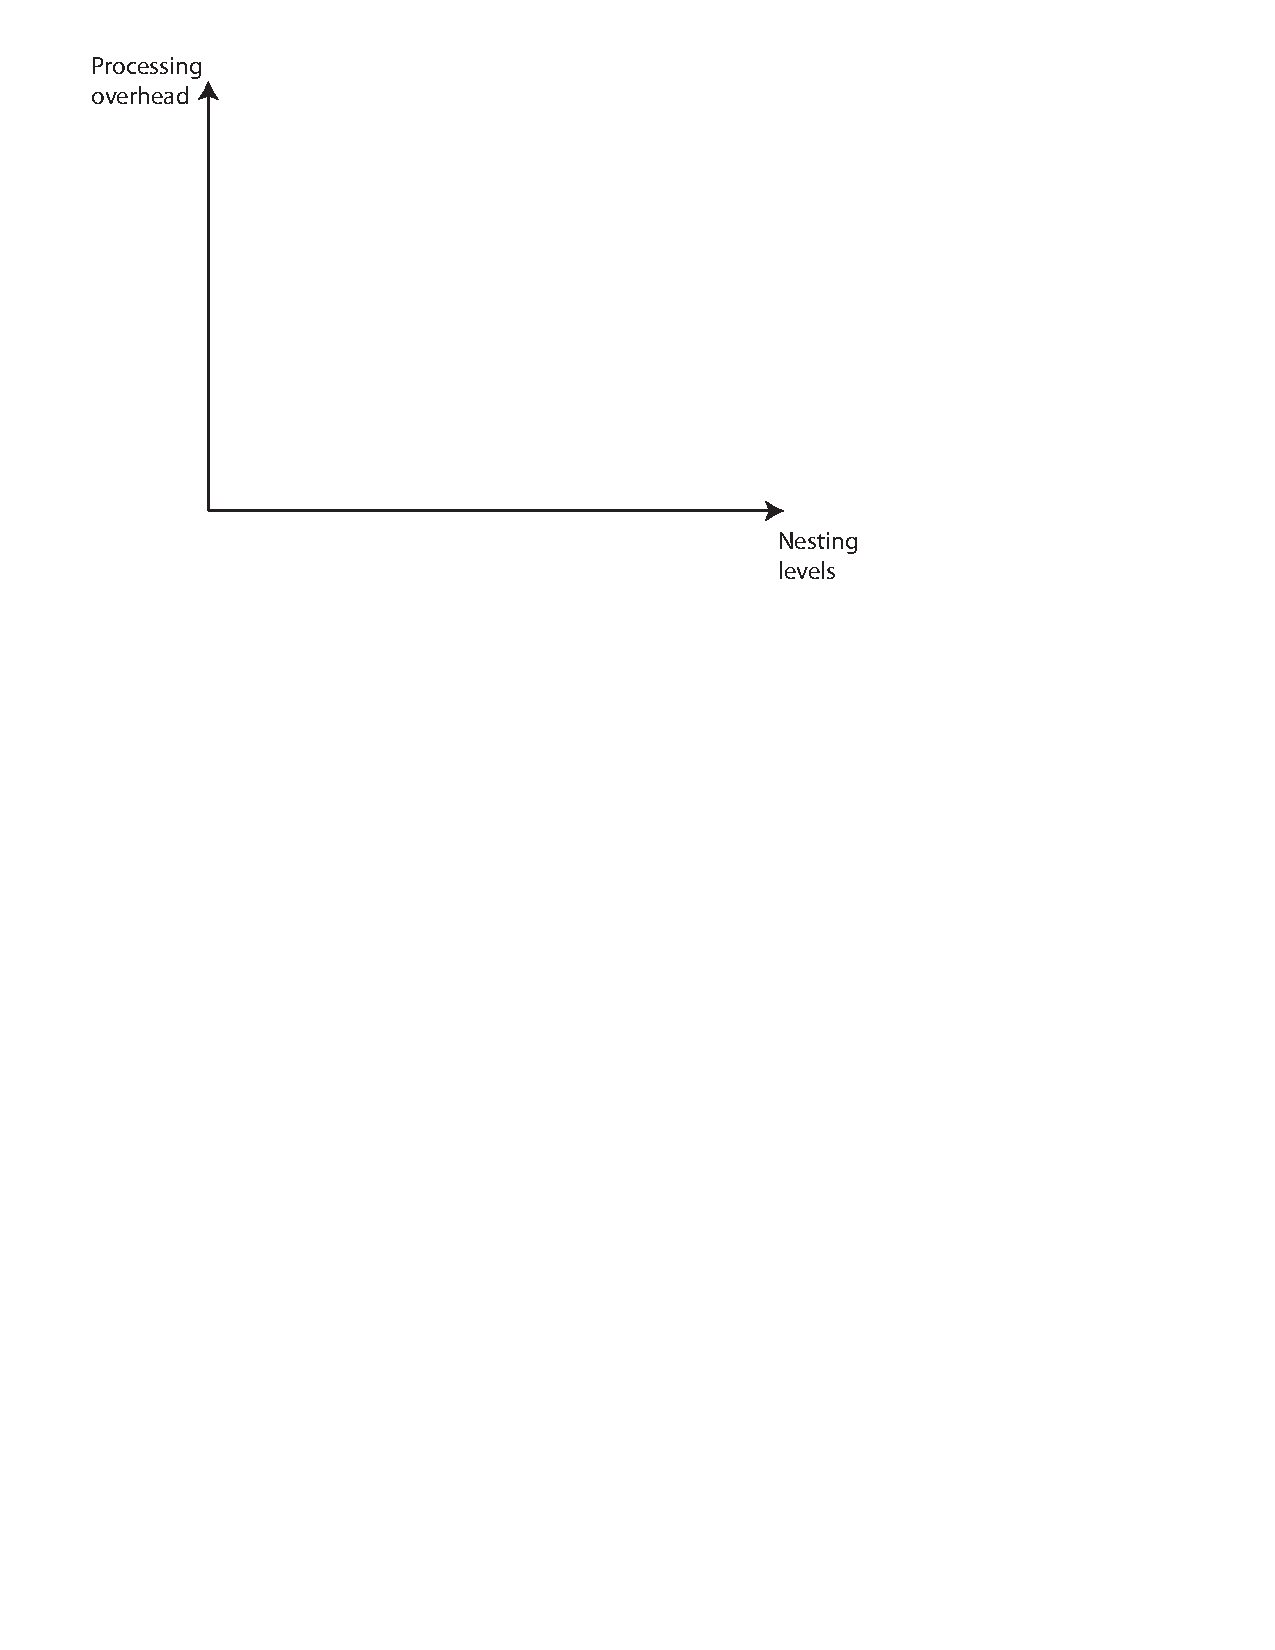
\includegraphics[scale=0.6]{figures/axes-nlevels.pdf}
\caption{Query processing overhead under varying nesting workloads, for
recursive compilation and incremental view maintenance.}
\label{fig:overhead-workload-nesting}
\end{figure}

\begin{figure}
\includegraphics[scale=0.6]{figures/axes-jgraph.pdf}
\caption{Query processing overhead under varying join graph workloads for
recursive compilation and incremental view maintenance.}
\label{fig:overhead-workload-join}
\end{figure}

\subsubsection{Algorithmic Trading and Data Warehousing applications}
\begin{itemize}
\item Compare naive query processing and incremental view maintenance to full
DBToaster recursive compilation for real-world scenarios.
\end{itemize}

\begin{figure}
\includegraphics[scale=0.6]{figures/axes-query.pdf}
\caption{Query processing overheads for the VWAP and SSB queries, for naive
  query processing, incremental view maintenance and DBToaster.}
\label{fig:overhead-vwap-ssb}
\end{figure}

\subsection{Memory Utilization}
\begin{itemize}
\item Measure total process memory usage over time, taking samples every $k$
  tuples (find a suitable value of $k$, perhaps 1000?).
\item Use the following formula to estimate a std::map$<>$ memory usage:
\begin{align*}
(sizeof(key) & + sizeof(value) + \\
& sizeof(rb\_tree\_node))*N\\
+ sizeof(rb\_tree)
\end{align*}

\item If time permits, use a custom allocator with an identifier for each map
assigned to use the allocator to track memory usage per map.

\item We have the following formulae for the number of maps created for k-way
joins with specific types of join graphs. These are derived by considering the
combinations of subgraphs of size $i$ (which constitute relations we can
aggregate), with $i = [1 \ldots k-1]$
    \begin{itemize}
    \item Chain: $\sum_{i=1}^{k}{i} = \frac{k(k+1)}{2}$
    \item Star: $(\sum_{i=1}^{k-1}{\binom{k-1}{i}}) + k $
    \item Cycle: $k*\sum_{i=1}^{k-1}{i} = \frac{k^2(k-1)}{2}$
    \end{itemize}

\item Predicted memory utilization:
    \begin{itemize}
    \item VWAP: mem(DBToaster) $>$ mem(VM) $>$ mem(naive) -- due to increased
    map usage, while still needing to maintain full domain. This changes if the base
    relation contains many duplicates, i.e. $|dom(P)| << |bids|$.
    \end{itemize}
\end{itemize}

\begin{figure}
\includegraphics[scale=0.6]{figures/axes-memnjquery.pdf}
\caption{Memory utilization of the naive, incremental view maintenance, and
  DBToaster query processing techniques on nested and multiway join queries.}
\label{fig:memutil-njquery}
\end{figure}

\begin{figure}
\includegraphics[scale=0.6]{figures/axes-memvsquery.pdf}
\caption{Memory utilization of the naive, incremental view maintenance, and
DBToaster query processing techniques for the VWAP and SSB queries.}
\label{fig:memutil-vsquery}
\end{figure}

\subsection{DBMS Bakeoff}
\begin{itemize}
\item Compare DBToaster to Postgres, HSQLDB, Oracle (DBMS 'X'), Borealis,
  Streambase (DBMS 'Y').
\item Compare using four different techniques: repetitive processing, trigger
  processing, builtin view maintenance, and stream processing.
\item What about a column store, e.g. Vertica/MonetDB? This would only be
  possible under a repetitive QP technique (or does Vertica implement triggers?)
\end{itemize}

\subsubsection{Repetitive Processing}
\begin{itemize}
\item Check whether we can simply pass through queries to Postgres, DBMS 'X' and
  HSQLDB, or whether it's better to generate from map algebra due to specific
  SQL syntax for each DBMS.
\item Run experiment for repeating at various fractions of the dataset size,
  i.e. 10\%,20\%,...,100\%, where 100\% means running the query for every tuple.
\item Note other DBMS can exploit caching here significantly, while DBToaster
  currently does not perform caching, and is L1/L2 cache-agnostic.
\end{itemize}

\begin{figure}
\includegraphics[scale=0.6]{figures/axes-repetitive.pdf}
\caption{Comparison of repetitive ad-hoc query processing of the VWAP and SSB
queries, in Postgres, DBMS 'X' and HSQLDB, to DBToaster's compiled query
processing.}
\label{fig:overhead-repetition}
\end{figure}

\subsubsection{Trigger-based processing}
\begin{itemize}
\item Generate trigger code from map algebra: use temporary tables as maps, and
  generate trigger code corresponding to each handler function.
\item HSQLDB only has Java-based triggers. Let's skip generating such Java-based
  triggers for now.
\item Postgres only allows row-based triggers to inspect tuple contents, DBMS
  'X' may allow access to the old and new tuple sets, allowing set-based
  triggering (like SQL Server).
\end{itemize}

\begin{figure}
\includegraphics[scale=0.6]{figures/axes-triggers.pdf}
\caption{Comparison of trigger-based processing of the VWAP and SSB queries in
Postgres, DBMS 'X' and HSQLDB to DBToaster's compiled query processing}
\label{fig:overhead-trigger}
\end{figure}

\subsubsection{Materialized view maintenance}
\begin{itemize}
\item Pick a feasible query for view maintenance (perhaps TPCH/SSB queries...) since
  VWAP cannot be done via incremental view maintenance in DBMS 'X'.
\item Check if we can simply pass through user-specified query to DBMS 'X's create
  view DDL statement.
\end{itemize}

\begin{figure}
\includegraphics[scale=0.6]{figures/axes-views.pdf}
\caption{Comparison of view maintenance in DBMS 'X' to DBToaster's compiled query processing}
\label{fig:overhead-trigger}
\end{figure}

\subsubsection{Stream processing}
\begin{itemize}
\item Pick a feasible query for stream processing (i.e., pure stream processing
  query, perhaps Linear Road avg lav), that does not require the use of
  in-memory tables.
\item Compare both VWAP query and pure-stream query (i.e. with windowing
  expressed as a range predicate in DBToaster).
\item Generate Borealis XML representation and Streambase app XML representation
  directly from initial map algebra.
\end{itemize}

\begin{figure}
\includegraphics[scale=0.6]{figures/axes-streams.pdf}
\caption{Comparison of stream processing implementations of the XXX query, for
  Borealis and DBMS 'Y' to DBToaster's compiled query processing.}
\label{fig:overhead-stream}
\end{figure}

\subsection{DBToaster Cost Model}

\section{Related Work}

\section{Conclusions}

\end{document}